\documentclass{article}

%package setup
\usepackage{graphicx}
\usepackage{amsmath}
\usepackage{fancyhdr}
\usepackage[margin=1in]{geometry}
\usepackage{comment}
\usepackage{placeins}
\usepackage{parskip}
\usepackage{subcaption}
\usepackage{appendix}
\usepackage{soul}
\usepackage{comment}
\PassOptionsToPackage{hyphens}{url}\usepackage[hidelinks]{hyperref}
\usepackage{matlab-prettifier}
\usepackage{minted}
\usepackage{enumitem}
\usepackage{float}
\usepackage{textcomp, gensymb}
\usepackage{tikz}
\usetikzlibrary{arrows.meta, positioning, decorations.pathmorphing}
\usepackage{caption}


\pagestyle{fancy}
\fancyhf{} % Clear header/footer settings
\rhead{\thepage} % Page number on the right in the header
\lhead{ASE162M Lab Report 1} % Your lab report title on the left

\begin{document}

\begin{titlepage}
  \centering
  \includegraphics[width=10cm]{ase-logo-formal.png}  % Adjust the width as needed
  \vspace{1cm}  % Add some vertical space
 
  \Large \textbf{ASE 162M High-Speed Aerodynamics}\\
  \large \textbf{Section 14275}\\
  \vspace{0.5cm}
  \textbf{Tuesay: 4:00 - 6:00 pm}\\
 
  \vspace{1cm}
 
  \hrule
  \vspace{0.5cm}
 
  \Huge \textbf{Report 1:\\
    Supersonic Flow over a Sphere}\\
  \Huge \textbf{}\\
 
  \vspace{0.5cm}
  \hrule
 
  \vspace{1cm}
 
  \normalsize \textbf{Andrew Doty}\\
  \normalsize \textbf{Due Date: 10/15/2024}
 
\end{titlepage}
\newpage

\tableofcontents
\thispagestyle{empty}
\newpage


\section{Introduction}

Supersonic flow over blunt bodies is a fundamental problem in compressible aerodynamics, with significant implications for the design of high-speed aircraft, spacecraft re-entry vehicles, and projectiles. When a supersonic flow encounters a blunt object such as a sphere, it forms a detached bow shock upstream of the body. The characteristics of this shock, particularly its standoff distance from the body, are crucial parameters in understanding the aerodynamic forces, heat transfer, and pressure distribution on the object.

The primary objective of this laboratory experiment is to investigate the behavior of supersonic flow over a sphere across a range of Mach numbers. Specifically, we aim to:

\begin{enumerate}
    \item Visualize the flow field and shock structure using Schlieren and shadowgraph imaging techniques.
    \item Measure and analyze the non-dimensional shock standoff distance as a function of Mach number.
    \item Compare experimental results with theoretical predictions through curve fitting of empirical relations.
    \item Examine the effects of Mach number and Reynolds number on the flow characteristics.
\end{enumerate}

The experiment utilizes the Aerolab Variable Mach Number Wind Tunnel, capable of producing flows with Mach numbers ranging from 1.4 to 3.5. A sphere model is mounted in the test section, and flow visualization is achieved using a folded Schlieren system with a pulsed xenon arc lamp. Pressure measurements in the stagnation chamber and test section provide data for calculating flow parameters.

This report presents the experimental methodology, data analysis, and discussion of results. We will examine the Schlieren images to identify key flow features, calculate Reynolds numbers and Mach numbers for each test condition, and analyze the shock standoff distance data. Three curve-fitting models will be applied to the standoff distance measurements:
\begin{enumerate}
    \item A qualitative scaling relation: $\frac{\delta}{D} = c\sqrt{\frac{1 + \frac{\gamma - 1}{2}M_\infty^2}{M_\infty - 1}}$
    \item A basic power-law fit: $\frac{\delta}{D} = c\gamma^\alpha M^\beta$
    \item An offset power-law fit: $\frac{\delta}{D} = c\gamma^\alpha (M - 1)^\beta$
\end{enumerate}

By comparing these models, we aim to gain insights into the physical mechanisms governing shock standoff distance and evaluate the applicability of different theoretical approaches.

The findings of this experiment contribute to our understanding of supersonic flow phenomena and provide valuable data for validating computational fluid dynamics (CFD) simulations and theoretical models. Such knowledge is essential for advancing the design and optimization of supersonic and hypersonic vehicles, as well as for predicting aerodynamic heating and loads in high-speed flight regimes.


\section{Experimental Setup}

The experiment was conducted using the Aerolab Variable Mach Number Wind Tunnel, capable of producing supersonic flows with Mach numbers ranging from approximately 1.63 to 3.25. The test section of the wind tunnel is nominally 3" * 3". A sphere model was mounted in the test section at a 0° angle of attack.

\subsection{Calibration and Imaging}

Prior to running the experiments, a calibration process was performed:

\begin{itemize}
    \item A 30/30, 5mm grid points calibration sheet was used for spatial calibration.
    \item 10 grid spaces, equivalent to 50mm, were used to determine the pixel-to-length ratio and associated uncertainty.
    \item A blank image without the calibration sheet was taken, followed by an image with the calibration sheet in place.
\end{itemize}

Flow visualization was achieved using both shadowgraph and Schlieren imaging techniques. A folded Schlieren system utilizing a pulsed xenon arc lamp as the light source was employed. For each Mach number, three types of images were captured:

\begin{enumerate}
    \item Shadowgraph
    \item Vertical Schlieren
    \item Horizontal Schlieren
\end{enumerate}

For the Schlieren setup, a knife edge was placed at the focal point to enhance the visualization of density gradients. The vertical and horizontal indicate the orientation of the blade. 

% \begin{tikzpicture}[scale=0.8]
%     % Wind tunnel
%     \draw[thick] (-5,2) -- (-3,2) to[out=0,in=180] (-1,1) to[out=0,in=180] (1,2) -- (7,2);
%     \draw[thick] (-5,-2) -- (-3,-2) to[out=0,in=180] (-1,-1) to[out=0,in=180] (1,-2) -- (7,-2);
   
%     % Sphere and bow shock
%     \fill[gray] (2,0) circle (0.2);
%     \draw[thick] (2,0) -- (7,0);  % Support rod
%     \draw[thick, red] (1.4,0.6) to[out=180,in=90] (1.2,0) to[out=-90,in=180] (1.4,-0.6);  % Bow shock
   
%     % Data acquisition boxes
%     \node[draw, minimum width=1cm, minimum height=0.8cm] at (9,1) {PT};
%     \node[draw, minimum width=1cm, minimum height=0.8cm] at (9,0) {DAQ};
%     \node[draw, minimum width=1cm, minimum height=0.8cm] at (9,-1) {PC};
   
%     % Pressure tubes
%     \draw[thick] (-4.5,-2) -- (-4.5,-2.5) -- (8.5,-2.5) -- (8.5,1) -- (8.7,1);
%     \node at (-4.5,-1.8) {P0};
   
%     \draw[thick] (3,-2) -- (3,-2.3) -- (8.3,-2.3) -- (8.3,1) -- (8.7,1);
%     \node at (3,-1.8) {P1};
   
%     % Camera
%     \draw[thick] (-0.5,-5) rectangle (0.5,-7);
%     \node at (0,-7.5) {Camera};
   
%     % Cable from PC to camera
%     \draw[thick] (9,-1) -- (9,-6) -- (0.5,-6);
   
%     % Labels
%     \node at (1,-2.8) {Wind Tunnel};
%     \node[red] at (0.8,0.8) {Bow Shock};
%     \node at (2.5,-0.5) {Sphere};
   
%     % Concave mirrors
%     \draw[thick] (0,3) to[out=10,in=170] (4,3);
%     \draw[thick] (0,-3) to[out=-10,in=-170] (4,-3);
   
%     % Vertical light paths
%     \foreach \x in {0.5,1.5,2.5,3.5}
%     {
%         \draw[thin] (\x,3) -- (\x,-3);
%     }
    
%     % Pulsed light source with converging lines
%     \draw[thick] (-5,4) rectangle (-4,3);
%     \node at (-4.5,3.5) {Pulsed};
%     \node at (-4.5,3.2) {Source};
%     \draw[thin] (-4,3.7) -- (-2,3);
%     \draw[thin] (-4,3.3) -- (-2,3);
    
%     % Dummy mirror
%     \draw[thick] (-2,4) to[out=-10,in=170] (0,4);
    
%     % Pinhole
%     \fill[black] (-2,3) circle (0.05);
%     \node at (-2,2.7) {Pinhole};
    
%     % Color filter
%     \draw[thick] (-1,4) rectangle (-0.5,3);
%     \node[rotate=90] at (-0.75,3.5) {Color filter};
    
%     % Knife edge
%     \draw[thick] (1.9,-3.5) -- (2.1,-3.5) -- (2,-3.3) -- cycle;
%     \node at (2,-3.8) {Knife edge};
    
%     % Focal point
%     \fill[black] (2,-3) circle (0.05);
%     \node at (2.5,-3) {Focal point};
% \end{tikzpicture}

% \begin{tikzpicture}[scale=0.8]
%     % Wind tunnel
%     \draw[thick] (-5,2) -- (-3,2) to[out=0,in=180] (-1,1) to[out=0,in=180] (1,2) -- (7,2);
%     \draw[thick] (-5,-2) -- (-3,-2) to[out=0,in=180] (-1,-1) to[out=0,in=180] (1,-2) -- (7,-2);
    
%     % Sphere and bow shock
%     \fill[gray] (2,0) circle (0.2);
%     \draw[thick] (2,0) -- (7,0);  % Support rod
%     \draw[thick, red] (1.4,0.6) to[out=180,in=90] (1.2,0) to[out=-90,in=180] (1.4,-0.6);  % Bow shock
    
%     % Data acquisition boxes
%     \node[draw, minimum width=1cm, minimum height=0.8cm] at (9,1) {PT};
%     \node[draw, minimum width=1cm, minimum height=0.8cm] at (9,0) {DAQ};
%     \node[draw, minimum width=1cm, minimum height=0.8cm] at (9,-1) {PC};
    
%     % Pressure tubes
%     \draw[thick] (-4.5,-2) -- (-4.5,-2.5) -- (8.5,-2.5) -- (8.5,1) -- (8.7,1);
%     \node at (-4.5,-1.8) {P0};
    
%     \draw[thick] (3,-2) -- (3,-2.3) -- (8.3,-2.3) -- (8.3,1) -- (8.7,1);
%     \node at (3,-1.8) {P1};
    
%     % Camera
%     \draw[thick] (-0.5,-5) rectangle (0.5,-7);
%     \node at (0,-7.5) {Camera};
    
%     % Cable from PC to camera
%     \draw[thick] (9,-1) -- (9,-6) -- (0.5,-6);
    
%     % Labels
%     \node at (1,-2.8) {Wind Tunnel};
%     \node[red] at (0.8,0.8) {Bow Shock};
%     \node at (2.5,-0.5) {Sphere};
    
%     % Concave mirrors
%     \draw[thick] (0,3) to[out=10,in=170] (4,3);
%     \draw[thick] (0,-3) to[out=-10,in=-170] (4,-3);
    
%     % Vertical light paths
%     \foreach \x in {0.5,1.5,2.5,3.5}
%     {
%         \draw[thin] (\x,3) -- (\x,-3);
%     }
% \end{tikzpicture}

% \begin{tikzpicture}[scale=0.8]
%     % Wind tunnel
%     \draw[thick] (-5,2) -- (-3,2) to[out=0,in=180] (-1,1) to[out=0,in=180] (1,2) -- (7,2);
%     \draw[thick] (-5,-2) -- (-3,-2) to[out=0,in=180] (-1,-1) to[out=0,in=180] (1,-2) -- (7,-2);
   
%     % Sphere and bow shock
%     \fill[gray] (2,0) circle (0.2);
%     \draw[thick] (2,0) -- (7,0);  % Support rod
%     \draw[thick, red] (1.4,0.6) to[out=180,in=90] (1.2,0) to[out=-90,in=180] (1.4,-0.6);  % Bow shock
   
%     % Data acquisition boxes
%     \node[draw, minimum width=1cm, minimum height=0.8cm] at (9,1) {PT};
%     \node[draw, minimum width=1cm, minimum height=0.8cm] at (9,0) {DAQ};
%     \node[draw, minimum width=1cm, minimum height=0.8cm] at (9,-1) {PC};
   
%     % Pressure tubes
%     \draw[thick] (-4.5,-2) -- (-4.5,-2.5) -- (8.5,-2.5) -- (8.5,1) -- (8.7,1);
%     \node at (-4.5,-1.8) {P0};
   
%     \draw[thick] (3,-2) -- (3,-2.3) -- (8.3,-2.3) -- (8.3,1) -- (8.7,1);
%     \node at (3,-1.8) {P1};
   
%     % Camera
%     \draw[thick] (-0.5,-7) rectangle (0.5,-9);
%     \node at (0,-9.5) {Camera};
   
%     % Cable from PC to camera
%     \draw[thick] (9,-1) -- (9,-8) -- (0.5,-8);
   
%     % Labels
%     \node at (1,-2.8) {Wind Tunnel};
%     \node[red] at (0.8,0.8) {Bow Shock};
%     \node at (2.5,-0.5) {Sphere};
   
%     % Concave mirrors
%     \draw[thick] (0,5) to[out=10,in=170] (4,5);
%     \draw[thick] (0,-5) to[out=-10,in=-170] (4,-5);
   
%     % Vertical light paths
%     \foreach \x in {0.5,1.5,2.5,3.5}
%     {
%         \draw[thin] (\x,5) -- (\x,-5);
%     }
    
%     % Pulsed light source
%     \draw[thick] (-5,5.5) rectangle (-4,4.5);
%     \node[text width=1cm, align=center] at (-4.5,5) {Pulsed Source};
    
%     % Pinhole
%     \fill[black] (-3,5) circle (0.05);
%     \node[above] at (-3,5.1) {Pinhole};
    
%     % Color filter
%     \draw[thick] (-1,5.5) rectangle (-0.5,4.5);
%     \node[above] at (-0.75,5.6) {Color filter};
    
%     % Converging lines
%     \draw[thin] (-3,5) -- (-0.75,5);
%     \foreach \x in {0.5,1.5,2.5,3.5}
%     {
%         \draw[thin] (\x,5) -- (-0.75,5);
%     }
   
%     % Dummy mirror (pivoted to go from quadrant 1 to 3)
%     \draw[thick] (2,-3) -- (-2,-7);
%     \node[rotate=45] at (-0.5,-5.5) {Dummy mirror};
    
%     % Converging lines from focal point to dummy mirror (added)
%     \foreach \x in {-1.6,-1.2,-0.8,-0.4,0,0.4,0.8,1.2,1.6}
%     {
%         \draw[thin] (\x,-5) -- (0,-6.5);
%     }
    
%     % Knife edge (above camera)
%     \draw[thick] (-0.1,-6.7) -- (0.1,-6.7) -- (0,-6.5) -- cycle;
%     \node[right] at (0.1,-6.7) {Knife edge};
    
%     % Focal point (above camera)
%     \fill[black] (0,-6.5) circle (0.05);
%     \node[left] at (-0.1,-6.5) {Focal point};
    
%     % Lines from focal point to camera
%     \draw[thin] (0,-6.5) -- (-0.3,-7);
%     \draw[thin] (0,-6.5) -- (0.3,-7);
% \end{tikzpicture}

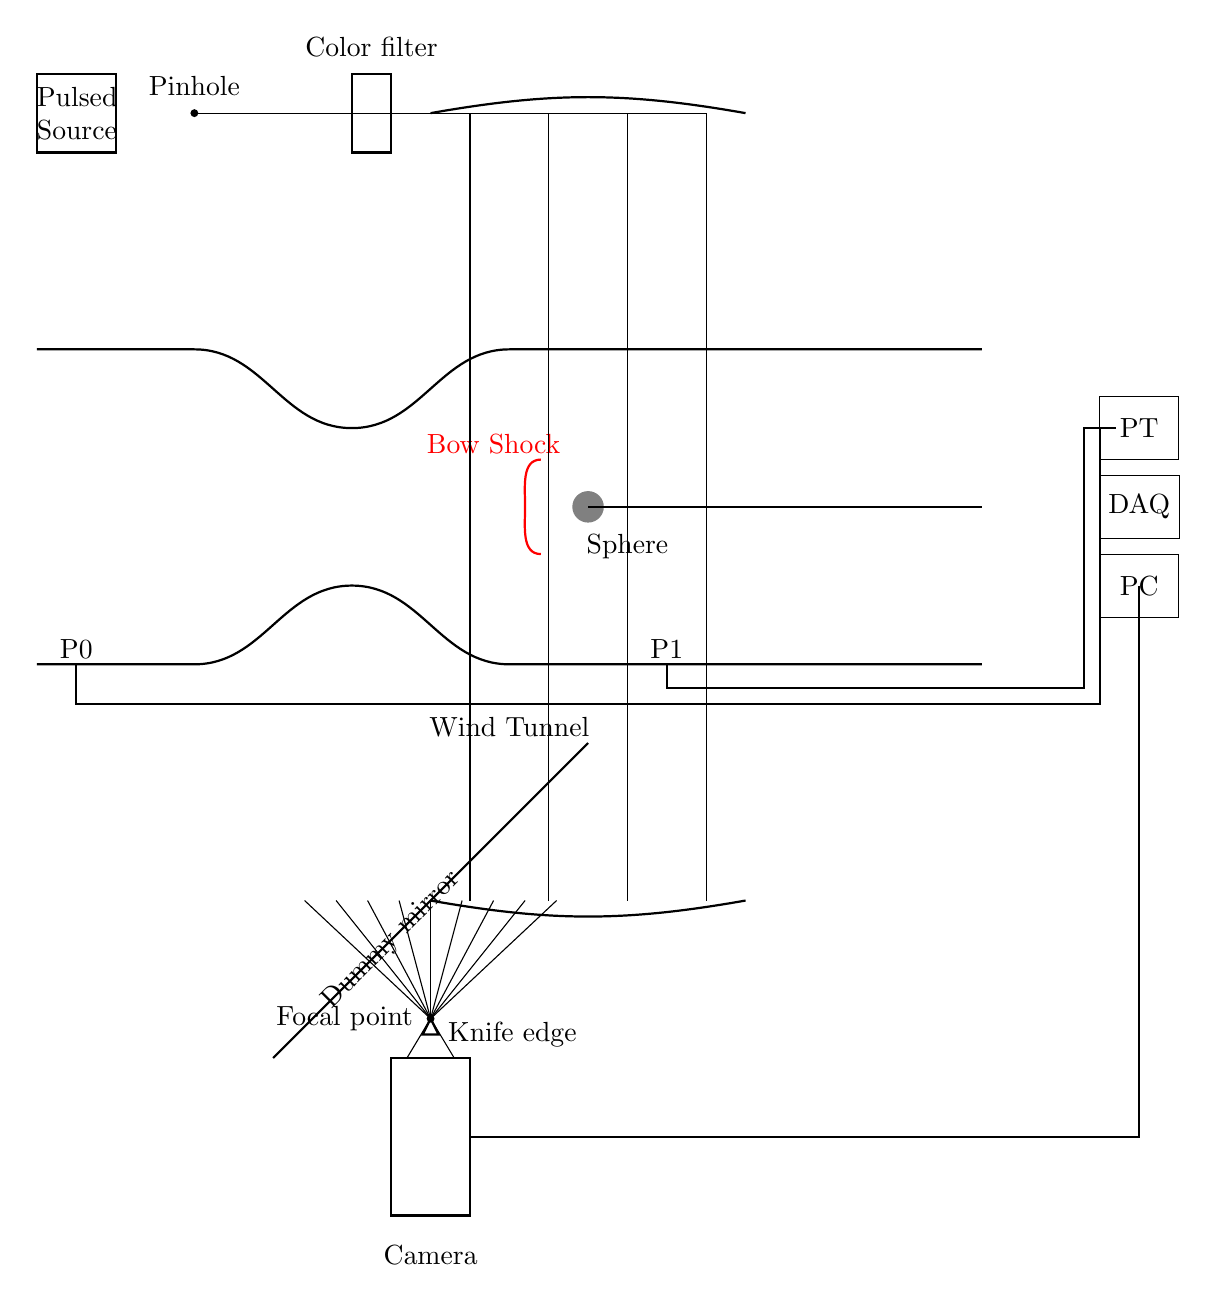
\begin{tikzpicture}[scale=1]
    % Wind tunnel
    \draw[thick] (-5,2) -- (-3,2) to[out=0,in=180] (-1,1) to[out=0,in=180] (1,2) -- (7,2);
    \draw[thick] (-5,-2) -- (-3,-2) to[out=0,in=180] (-1,-1) to[out=0,in=180] (1,-2) -- (7,-2);
   
    % Sphere and bow shock
    \fill[gray] (2,0) circle (0.2);
    \draw[thick] (2,0) -- (7,0);  % Support rod
    \draw[thick, red] (1.4,0.6) to[out=180,in=90] (1.2,0) to[out=-90,in=180] (1.4,-0.6);  % Bow shock
   
    % Data acquisition boxes
    \node[draw, minimum width=1cm, minimum height=0.8cm] at (9,1) {PT};
    \node[draw, minimum width=1cm, minimum height=0.8cm] at (9,0) {DAQ};
    \node[draw, minimum width=1cm, minimum height=0.8cm] at (9,-1) {PC};
   
    % Pressure tubes
    \draw[thick] (-4.5,-2) -- (-4.5,-2.5) -- (8.5,-2.5) -- (8.5,1) -- (8.7,1);
    \node at (-4.5,-1.8) {P0};
   
    \draw[thick] (3,-2) -- (3,-2.3) -- (8.3,-2.3) -- (8.3,1) -- (8.7,1);
    \node at (3,-1.8) {P1};
   
    % Camera
    \draw[thick] (-0.5,-7) rectangle (0.5,-9);
    \node at (0,-9.5) {Camera};
   
    % Cable from PC to camera
    \draw[thick] (9,-1) -- (9,-8) -- (0.5,-8);
   
    % Labels
    \node at (1,-2.8) {Wind Tunnel};
    \node[red] at (0.8,0.8) {Bow Shock};
    \node at (2.5,-0.5) {Sphere};
   
    % Concave mirrors
    \draw[thick] (0,5) to[out=10,in=170] (4,5);
    \draw[thick] (0,-5) to[out=-10,in=-170] (4,-5);
   
    % Vertical light paths
    \foreach \x in {0.5,1.5,2.5,3.5}
    {
        \draw[thin] (\x,5) -- (\x,-5);
    }
   
    % Pulsed light source
    \draw[thick] (-5,5.5) rectangle (-4,4.5);
    \node[text width=1cm, align=center] at (-4.5,5) {Pulsed Source};
   
    % Pinhole
    \fill[black] (-3,5) circle (0.05);
    \node[above] at (-3,5.1) {Pinhole};
   
    % Color filter
    \draw[thick] (-1,5.5) rectangle (-0.5,4.5);
    \node[above] at (-0.75,5.6) {Color filter};
   
    % Converging lines (top)
    \draw[thin] (-3,5) -- (-0.75,5);
    \foreach \x in {0.5,1.5,2.5,3.5}
    {
        \draw[thin] (\x,5) -- (-0.75,5);
    }
   
    % Dummy mirror (pivoted to go from quadrant 1 to 3)
    \draw[thick] (2,-3) -- (-2,-7);
    \node[rotate=45] at (-0.5,-5.5) {Dummy mirror};
   
    % Converging lines from focal point to dummy mirror (added)
    \foreach \x in {-1.6,-1.2,-0.8,-0.4,0,0.4,0.8,1.2,1.6}
    {
        \draw[thin] (\x,-5) -- (0,-6.5);
    }
   
    % Knife edge (above camera)
    \draw[thick] (-0.1,-6.7) -- (0.1,-6.7) -- (0,-6.5) -- cycle;
    \node[right] at (0.1,-6.7) {Knife edge};
   
    % Focal point (above camera)
    \fill[black] (0,-6.5) circle (0.05);
    \node[left] at (-0.1,-6.5) {Focal point};
   
    % Lines from focal point to camera
    \draw[thin] (0,-6.5) -- (-0.3,-7);
    \draw[thin] (0,-6.5) -- (0.3,-7);
\end{tikzpicture}

Note for Ryan, this was my first tikz diagram of this type, and I am still learning so please don't grade me too harshly :)

\subsection{Data Acquisition}

Pressure measurements were recorded using a LabVIEW-based data acquisition system. Two pressure transducers were used:

\begin{itemize}
    \item Channel 0: Stagnation pressure (P\textsubscript{0})
    \item Channel 1: Freestream static pressure
\end{itemize}

The pressure data was recorded in volts (gauge pressure) and later converted to appropriate units using calibration constants.

\subsection{Experimental Procedure}

The experiment followed these steps for each run:

\begin{enumerate}
    \item The wind tunnel was started in the sequence: power, hydraulic, then run.
    \item The initial Mach number was set to approximately 3, with subsequent runs decreasing by increments of 0.25.
    \item Once the LabVIEW system showed stable pressure readings, images were captured using the Pulnix color CCD camera and XCAP for Windows acquisition software.
    \item The wind tunnel was operated only while the run button was held, and shut down in the reverse order of startup once the airflow stopped.
    \item Mach number was adjusted by changing the area ratio and chamber pressure according to the manufacturer's specifications, referencing the "Approximate Minimum Stagnation Pressure vs Mach Number" chart.
\end{enumerate}

Care was taken to monitor the pressure of the compressed air tank to ensure consistent flow quality across all runs. The experiment was repeated for Mach numbers of 3, 2.75, 2.5, 2.25, 2, and 1.75.


\section{Results and Discussion}

\subsection{Reynolds Number and Mach Number Calculations}

To calculate the Reynolds numbers and Mach numbers, we used the following equations:

\subsubsection{Mach Number Calculation}
The Mach number was calculated using the isentropic flow equation:

\begin{equation}
    \frac{p_0}{p} = \left(1 + \frac{\gamma - 1}{2} M^2\right)^{\frac{\gamma}{\gamma - 1}}
\end{equation}

where $p_0$ is the stagnation pressure, $p$ is the static pressure, $\gamma$ is the ratio of specific heats for air (1.4), and $M$ is the Mach number.

\subsubsection{Reynolds Number Calculation}
The Reynolds numbers were calculated using:

\begin{equation}
    Re_D = \frac{\rho_\infty U_\infty D}{\mu}
\end{equation}

where $\rho_\infty$ is the freestream density, $U_\infty$ is the freestream velocity, $D$ is the sphere diameter, and $\mu$ is the dynamic viscosity.

The viscosity was calculated using Sutherland's law:

\begin{equation}
    \mu = \mu_0 \left(\frac{T}{T_0}\right)^{3/2} \frac{T_0 + C}{T + C}
\end{equation}

where $\mu_0$ is the reference viscosity, $T_0$ is the reference temperature, $T$ is the flow temperature, and $C$ is Sutherland's constant for air.

Using the data from the pressure measurements and the Python script, we calculated the unit Reynolds numbers and diametric Reynolds numbers ($Re_D$) for all runs, as well as the Mach numbers. Sutherland's law was used for viscosity calculations. The results are presented in the following plot:
\begin{figure}[H]
\centering
\includegraphics[width=0.8\textwidth]{Mach-Number-vs-Reynolds.png}
\caption{Mach number vs. Diametric Reynolds number}
\label{fig:mach_vs_red}
\end{figure}

Figure \ref{fig:mach_vs_red} shows the relationship between the calculated Mach number and the diametric Reynolds number. We observe a positive correlation, with both Mach number and Reynolds number increasing together. This trend is expected due to higher flow velocities at increased Mach numbers.

The error bars represent propagated uncertainties from measurement errors. For Mach number, the uncertainty is primarily due to pressure measurement errors:

\begin{equation}
    \delta M = \sqrt{\left(\frac{\partial M}{\partial p_0}\delta p_0\right)^2 + \left(\frac{\partial M}{\partial p}\delta p\right)^2}
\end{equation}

where $\delta p_0$ and $\delta p$ are uncertainties in stagnation and static pressure measurements, respectively.

For Reynolds number, uncertainties propagate from multiple sources:

\begin{equation}
    \delta Re_D = Re_D \sqrt{\left(\frac{\delta \rho}{\rho}\right)^2 + \left(\frac{\delta U}{U}\right)^2 + \left(\frac{\delta D}{D}\right)^2 + \left(\frac{\delta \mu}{\mu}\right)^2}
\end{equation}

where $\delta \rho$, $\delta U$, $\delta D$, and $\delta \mu$ are uncertainties in density, velocity, diameter, and viscosity calculations, respectively.

The increasing size of error bars at higher Mach and Reynolds numbers indicates that measurement uncertainties have a more significant impact in these regimes, likely due to the nonlinear relationships in the governing equations.


\subsection{Schlieren Images Analysis}
We analyzed the Schlieren images for the highest and lowest Mach numbers to observe the flow features around the sphere.
\begin{figure}[H]
\centering
\begin{subfigure}[b]{0.45\textwidth}
\includegraphics[width=\textwidth]{lowest_mach.png}
\caption{Lowest Mach number Horizontal(M = 1.75)}
\label{fig:lowest_mach}
\end{subfigure}
\begin{subfigure}[b]{0.45\textwidth}
    \includegraphics[width=\textwidth]{lowest_mach_vertical.png}
    \caption{Lowest Mach number Vertical (M = 1.75)}
    \label{fig:lowest_mach_vertical}
    \end{subfigure}
\hfill
\begin{subfigure}[b]{0.45\textwidth}
\includegraphics[width=\textwidth]{highest_mach_horizontal.png}
\caption{Highest Mach number Horizontal (M = 3.0)}
\label{fig:highest_mach}
\end{subfigure}
\begin{subfigure}[b]{0.45\textwidth}
    \includegraphics[width=\textwidth]{highest_mach_vertical.png}
    \caption{Highest Mach number Vertical(M = 3.0)}
    \label{fig:highest_mach_vertical}
\end{subfigure}
\caption{Schlieren images at extreme Mach numbers}
\label{fig:schlieren_images}
\end{figure}

In Figure \ref{fig:schlieren_images}, we can observe the following key features:
\begin{enumerate}
    \item Bow shock: A strong, detached shock wave is visible in front of the sphere for both Mach numbers. The shock is more oblique and closer to the sphere at the higher Mach number.
    \item Shock standoff distance: The distance between the bow shock and the sphere's leading edge is noticeably larger for the lower Mach number (Figure \ref{fig:lowest_mach}) compared to the higher Mach number (Figure \ref{fig:highest_mach}).
    \item Expansion region: Behind the sphere, we can see an expansion fan where the flow accelerates and turns around the sphere.
    \item Wake region: A turbulent wake is visible downstream of the sphere, characterized by density gradients in the Schlieren images.
    \item Boundary layer: Although not clearly visible due to the image resolution, a thin boundary layer is expected to form on the sphere's surface.
\end{enumerate}
The changes in the flow structure as the Mach number increases from 1.75 to 3.0 are consistent with theory:
\begin{enumerate}
    \item The bow shock moves closer to the sphere at higher Mach numbers, reducing the shock standoff distance.
    \item The shock becomes stronger and more oblique at higher Mach numbers, as evidenced by the sharper contrast in the Schlieren image.
    \item The wake region appears to be more compressed and elongated at the higher Mach number, likely due to the increased dynamic pressure.
    \item These changes correlate with the increase in Reynolds number observed in Figure \ref{fig:mach_vs_red}.
\end{enumerate}



\subsection{Shock Standoff Distance Analysis}

We analyzed the non-dimensional shock standoff distance $\delta/D$ as a function of Mach number using the formula:
\begin{equation}
\frac{\delta}{D} = f(M)
\end{equation}
where $\delta$ is the shock standoff distance and $D$ is the sphere diameter. The standoff distance $\delta$ and sphere diameter $D$ were measured using a custom image analysis script developed for this experiment. This script processes the Schlieren images, allowing for precise measurement of the shock location and sphere dimensions. The visual can be shown below.

\begin{figure}[H]
\centering
\includegraphics[width=0.8\textwidth]{delta_over_d.png}
\caption{Non-dimensional standoff distance vs. Mach number}
\label{fig:delta_vs_mach}
\end{figure}

Figure \ref{fig:delta_vs_mach} presents the relationship between the non-dimensional standoff distance and Mach number. The graph reveals several key observations:

\begin{itemize}
    \item Inverse relationship: As the Mach number increases, the non-dimensional standoff distance decreases, consistent with our Schlieren image observations and theoretical expectations.
    \item Nonlinear trend: The relationship appears nonlinear, with a steeper decrease in standoff distance at lower Mach numbers (1.75 to 2.25) and a more gradual decrease at higher Mach numbers (2.5 to 3.0).
    \item Range: The non-dimensional standoff distance ranges from approximately 0.24 at Mach 1.75 to 0.10 at Mach 3.0, representing a significant change in shock structure over the tested Mach number range.
    \item Asymptotic behavior: The curve shape suggests an asymptotic approach to a minimum standoff distance as Mach number increases, which aligns with theoretical predictions for hypersonic flow regimes.
\end{itemize}

This trend is explained by the physics of shock formation in supersonic flows. As the Mach number increases, the bow shock forms closer to the sphere due to the increased shock strength and more efficient flow compression.




\subsection{Curve Fitting}

We performed curve fitting on the standoff distance data using three different relations:

\subsubsection{Qualitative scaling dependence}
\begin{equation}
\frac{\delta}{D} = c\sqrt{\frac{1 + \frac{\gamma - 1}{2}M_\infty^2}{M_\infty - 1}}
\end{equation}
\subsubsection{Basic fit}
\begin{equation}
\frac{\delta}{D} = c\gamma^\alpha M^\beta
\end{equation}
\subsubsection{Offset fit}
\begin{equation}
\frac{\delta}{D} = c\gamma^\alpha (M - 1)^\beta
\end{equation}
The results of these curve fits are presented in the following plot and table:
\begin{figure}[H]
\centering
\includegraphics[width=0.8\textwidth]{delta_over_d-fits.png}
\caption{Curve fits for non-dimensional standoff distance}
\label{fig:curve_fits}
\end{figure}


\begin{table}[h]
\centering
\caption{Curve Fit Parameters}
\label{tab:curve_fit_params}
\begin{tabular}{lccc}
\hline
Fit Type & $c$ & $\alpha$ & $\beta$ \\
\hline
Qualitative & 0.2157 & N/A & N/A \\
Basic & 0.2315 & 9.448 & -1.635 \\
Offset & 0.1653 & -1.774 & -0.881 \\
\hline
\end{tabular}
\end{table}

\section{Discussion}
The data exhibits good agreement with all three relations, which can be characterized as follows:

\begin{enumerate}
    \item \textbf{Qualitative scaling}: 
       \begin{equation}
           \frac{\delta}{D} = c\sqrt{\frac{1 + \frac{\gamma - 1}{2}M_\infty^2}{M_\infty - 1}}
       \end{equation}
       This fit captures the general trend of decreasing standoff distance with increasing Mach number. The single parameter $c$ (0.2157) represents a scaling factor that accounts for the overall magnitude of the standoff distance. The qualitative scaling shows good agreement with the data, especially at higher Mach numbers, reflecting the physical expectation of asymptotic behavior as Mach number increases.
    
    \item \textbf{Basic fit}: 
       \begin{equation}
           \frac{\delta}{D} = c\gamma^\alpha M^\beta
       \end{equation}
       The negative value of $\beta$ (-1.635) confirms the inverse relationship between Mach number and standoff distance, aligning with physical expectations. The large positive value of $\alpha$ (9.448) suggests a strong dependence on the specific heat ratio $\gamma$. This is somewhat unexpected for a simple geometry like a sphere and may indicate that the fit is compensating for other factors not explicitly accounted for in the model.
    
    \item \textbf{Offset fit}: 
       \begin{equation}
           \frac{\delta}{D} = c\gamma^\alpha (M - 1)^\beta
       \end{equation}
       This fit attempts to account for the behavior near Mach 1 by using (M - 1) instead of M. The negative $\alpha$ (-1.774) and $\beta$ (-0.881) indicate that the standoff distance decreases with increasing Mach number, but at a different rate compared to the basic fit. The offset fit appears to provide a good balance between accuracy and physical interpretation, especially for lower Mach numbers.
\end{enumerate}

Regarding the dependence on composition (through $\gamma$) and Mach number:

\begin{enumerate}
    \item For the basic fit, the strong dependence on $\gamma$ (large $\alpha$) is unexpected. We would typically expect a weaker dependence on composition for a simple geometry like a sphere. This suggests that the fit might be overcompensating for other factors or that there may be additional physics not captured by this simple model.
    
    \item The offset fit shows a negative dependence on $\gamma$, which is also unexpected. However, the magnitude is smaller than in the basic fit, suggesting it might be a more realistic representation of the weak composition dependence we would expect.
    
    \item Both fits show a strong dependence on Mach number (through $\beta$), which aligns with my physical understanding of shock formation in supersonic flows. The offset fit's use of (M - 1) provides a better representation of the behavior near Mach 1, which is consistent with theoretical expectations.
\end{enumerate}

The consistency of our data with these fits is generally good, as evidenced by the close agreement between the fit curves and the experimental data points in Figure \ref{fig:curve_fits}. However, there are some discrepancies, particularly at Mach numbers around 2.25 and 2.75, where the experimental data points deviate slightly from all three fit curves.

\section{Conclusion}

This experiment explored supersonic flow over a sphere at Mach numbers from 1.75 to 3.0. We visualized the flow field using Schlieren imaging, analyzed the non-dimensional shock standoff distance, and compared experimental results with theoretical predictions through curve fitting.

The Mach number versus Reynolds number analysis showed a positive correlation, with higher uncertainties at higher Mach numbers. Schlieren images revealed the shock structure's dependence on Mach number, with the bow shock moving closer to the sphere at higher Mach numbers.

The non-dimensional standoff distance analysis, using three fitting methods (qualitative scaling, basic fit, and offset fit), provided unique insights into shock formation. The offset fit seemed to offer the best balance between accuracy and physical interpretation, especially near Mach 1.

Surprisingly, the basic and offset fits suggested a stronger dependence on gas composition than expected for a simple spherical geometry. This finding highlights the complexity of supersonic flow and the limitations of simplified models. It also suggests avenues for future research, such as exploring a wider range of Mach numbers or investigating the effects of different gas compositions on shock standoff distances.

Insights gained from this work contribute to the broader field of high-speed aerodynamics and may have implications for the design and optimization of supersonic and hypersonic vehicles. Future studies could build upon these findings to further refine our models and deepen our understanding of complex flow phenomena in high-speed regimes.

\appendix
\section{References}

\begin{enumerate}
    \item Anderson, J. D. (2010). Fundamentals of aerodynamics. Tata McGraw-Hill Education.
    \item Liepmann, H. W., \& Roshko, A. (1957). Elements of gasdynamics. John Wiley \& Sons.
    \item Van Dyke, M. (1982). An album of fluid motion. Parabolic Press.
\end{enumerate}

\section{Python Scripts}

\subsection{standoff2.py}

\begin{minted}{python}

\end{minted}

\subsection{mach-analysis.py}

\begin{minted}{python}
    import os
import re
import numpy as np
import matplotlib.pyplot as plt
from scipy.signal import find_peaks
from scipy.optimize import fsolve, curve_fit

def read_data_file(file_path):
    with open(file_path, 'r') as f:
        lines = f.readlines()
    
    data_start = next(i for i, line in enumerate(lines) if "X_Value" in line)
    data = np.genfromtxt(lines[data_start+1:], delimiter='\t', usecols=(1, 2))
    return data

def voltage_to_pressure(voltage, conversion_factor):
    return voltage * (conversion_factor / 0.1)

def find_steady_state(data, window_size=50):
    # Find the index of the maximum pressure
    peak_index = np.argmax(np.abs(data))
    
    # Define a region around the peak to search for the steady state
    search_start = max(0, peak_index - window_size*2)
    search_end = min(len(data), peak_index + window_size*2)
    
    # Calculate moving standard deviation
    std_dev = np.array([np.std(data[i:i+window_size]) for i in range(search_start, search_end-window_size)])
    
    # Find the region with the lowest standard deviation (most stable)
    stable_start = search_start + np.argmin(std_dev)
    
    return stable_start, stable_start + window_size

def calculate_mach_number(p0_gauge, p_gauge, p_atm=14.7, gamma=1.4):
    # Convert gauge pressures to absolute pressures
    p0 = p0_gauge + p_atm
    p = p_gauge + p_atm
    
    if p0 <= p or p <= 0:
        return np.nan
    
    # Use the correct isentropic flow equation for Mach number
    mach = np.sqrt((2 / (gamma - 1)) * ((p0 / p)**((gamma - 1) / gamma) - 1))
    
    return mach

def calculate_reynolds_numbers(mach_number, pressure, temperature, diameter):
    # Constants
    gamma = 1.4  # Ratio of specific heats for air
    R = 287.05  # Gas constant for air in J/(kg·K)
    
    # Sutherland's law constants
    C = 120  # Sutherland's constant for air in K
    T0 = 291.15  # Reference temperature in K
    mu0 = 1.827e-5  # Reference viscosity in Pa·s

    # Calculate temperature ratio
    T_ratio = 1 + (gamma - 1) / 2 * mach_number**2
    T = temperature * T_ratio  # Static temperature

    # Calculate density
    rho = pressure / (R * T)

    # Calculate velocity
    V = mach_number * np.sqrt(gamma * R * T)

    # Calculate viscosity using Sutherland's law
    mu = mu0 * (T / T0)**(3/2) * (T0 + C) / (T + C)

    # Calculate Reynolds numbers
    Re_unit = rho * V / mu
    Re_D = Re_unit * diameter

    return Re_unit, Re_D

def mach_number_uncertainty(p0, p, dp0, dp, gamma=1.4):
    # Function to solve for Mach number
    def mach_equation(M):
        return (p0/p) - (1 + (gamma-1)/2 * M**2)**(gamma/(gamma-1))

    # Calculate Mach number
    M = fsolve(mach_equation, 1.0)[0]

    # Partial derivatives
    dM_dp0 = M / (2*p0) * (1 + (gamma-1)/2 * M**2)
    dM_dp = -M / (2*p) * (1 + (gamma-1)/2 * M**2)

    # Uncertainty propagation
    dM = np.sqrt((dM_dp0 * dp0)**2 + (dM_dp * dp)**2)

    return M, dM

def process_file(file_path):
    data = read_data_file(file_path)
    
    stagnation_pressure = voltage_to_pressure(data[:, 0], 60)
    static_pressure = voltage_to_pressure(data[:, 1], 15)
    
    start, end = find_steady_state(stagnation_pressure)
    
    avg_stagnation_pressure = np.mean(stagnation_pressure[start:end])
    avg_static_pressure = np.mean(static_pressure[start:end])
    
    mach_number, mach_uncertainty = mach_number_uncertainty(avg_stagnation_pressure + 14.7, 
                                                            avg_static_pressure + 14.7, 
                                                            0.01 * avg_stagnation_pressure, 
                                                            0.01 * avg_static_pressure)
    
    # Calculate Reynolds numbers
    diameter = 0.0163  # Sphere diameter in meters
    Re_unit, Re_D = calculate_reynolds_numbers(mach_number, avg_static_pressure * 6894.75729,  # Convert psi to Pa
                                               297, diameter)  # Assuming 297 K (24°C) ambient temperature
    
    # Calculate Reynolds number uncertainty (simplified, assuming only Mach number contributes significantly)
    dRe_D = Re_D * mach_uncertainty / mach_number
    
    # Visualize the data
    # plt.figure(figsize=(12, 6))
    # plt.plot(stagnation_pressure, label='Stagnation Pressure')
    # plt.plot(static_pressure, label='Static Pressure')
    # plt.axvline(start, color='r', linestyle='--', label='Steady State Start')
    # plt.axvline(end, color='r', linestyle='--', label='Steady State End')
    # plt.axhline(avg_stagnation_pressure, color='g', linestyle=':', label='Avg Stagnation')
    # plt.axhline(avg_static_pressure, color='m', linestyle=':', label='Avg Static')
    # plt.legend()
    # plt.title(f'Pressure Data for {os.path.basename(file_path)}')
    # plt.xlabel('Sample')
    # plt.ylabel('Pressure (psi)')
    # plt.show()
    
    print(f"File: {os.path.basename(file_path)}")
    print(f"Stagnation Pressure (gauge): {avg_stagnation_pressure:.2f} psi")
    print(f"Static Pressure (gauge): {avg_static_pressure:.2f} psi")
    print(f"Stagnation Pressure (absolute): {avg_stagnation_pressure + 14.7:.2f} psi")
    print(f"Static Pressure (absolute): {avg_static_pressure + 14.7:.2f} psi")
    print(f"Pressure Ratio (p/p0): {(avg_static_pressure + 14.7) / (avg_stagnation_pressure + 14.7):.4f}")
    print(f"Calculated Mach Number: {mach_number:.2f}")
    print(f"Unit Reynolds Number: {Re_unit:.2e} 1/m")
    print(f"Diametric Reynolds Number: {Re_D:.2e}")
    print(f"Reynolds Number Uncertainty: {dRe_D:.2e}")
    print("---")
    
    return mach_number, mach_uncertainty, avg_stagnation_pressure, avg_static_pressure, Re_unit, Re_D, dRe_D

def extract_mach_number(filename):
    match = re.search(r'M(\d+)_(\d+)', filename)
    if match:
        return float(f"{match.group(1)}.{match.group(2)}")
    return None

# Directory containing the data files
data_dir = r"Lab 1\Working-data"

results = []

for filename in os.listdir(data_dir):
    if filename.endswith(".txt"):
        file_path = os.path.join(data_dir, filename)
        expected_mach = extract_mach_number(filename)
        if expected_mach:
            calculated_mach, mach_uncertainty, stagnation_p, static_p, Re_unit, Re_D, dRe_D = process_file(file_path)
            results.append((expected_mach, calculated_mach, mach_uncertainty, stagnation_p, static_p, Re_unit, Re_D, dRe_D))
            print(f"Processed {filename}: Expected M={expected_mach:.2f}, Calculated M={calculated_mach:.2f} ± {mach_uncertainty:.2f}")

# Sort results by expected Mach number
results.sort(key=lambda x: x[0])

# Plotting Mach number vs Re_D with error bars (vertical only)
plt.figure(figsize=(10, 6))
mach_numbers, re_d_numbers, re_d_uncertainties = zip(*[(calc_mach, re_d, dre_d) 
                                                       for _, calc_mach, _, _, _, _, re_d, dre_d in results])

# Use absolute values for uncertainties
re_d_uncertainties = np.abs(re_d_uncertainties)

plt.errorbar(mach_numbers, np.abs(re_d_numbers), yerr=re_d_uncertainties, fmt='o', capsize=5)
plt.xlabel('Mach Number')
plt.ylabel('Reynolds Number (Re_D)')
plt.title('Mach Number vs Reynolds Number with Uncertainties')
plt.grid(True)
plt.show()

# Print results
print("\nMach Number and Reynolds Number Comparison with Uncertainties:")
print("Expected M | Calculated M ± Uncertainty | Re_D ± Uncertainty")
print("-" * 70)
for expected, calculated, mach_unc, _, _, _, re_d, dre_d in results:
    print(f"{expected:.2f}       | {calculated:.2f} ± {abs(mach_unc):.2f}              | {re_d:.2e} ± {abs(dre_d):.2e}")

# Calculate and print average error
valid_results = [(exp, calc) for exp, calc, _, _, _, _, _, _ in results if not np.isnan(calc)]
if valid_results:
    errors = [abs(calc - exp) for exp, calc in valid_results]
    avg_error = np.mean(errors)
    print(f"\nAverage Mach number error: {avg_error:.4f}")
else:
    print("\nNo valid Mach number calculations.")

# Add these new functions after the existing functions

def calculate_nondimensional_standoff(mach_numbers, diameters, standoff_distances):
    return np.array(standoff_distances) / np.array(diameters)

def qualitative_scaling(M, c, gamma=1.4):
    return c * np.sqrt((1 + (gamma - 1) / 2 * M**2) / (M - 1))

def basic_fit(M, c, alpha, beta, gamma=1.4):
    return c * gamma**alpha * M**beta

def offset_fit(M, c, alpha, beta, gamma=1.4):
    return c * gamma**alpha * (M - 1)**beta

def plot_nondimensional_standoff(mach_numbers, nondimensional_standoff):
    plt.figure(figsize=(10, 6))
    plt.scatter(mach_numbers, nondimensional_standoff)
    plt.xlabel('Mach Number')
    plt.ylabel('δ/D')
    plt.title('Non-dimensional Standoff Distance vs Mach Number')
    plt.grid(True)
    plt.show()

def perform_curve_fits(mach_numbers, nondimensional_standoff):
    # Qualitative scaling fit
    popt_qual, _ = curve_fit(qualitative_scaling, mach_numbers, nondimensional_standoff)
    
    # Basic fit
    popt_basic, _ = curve_fit(basic_fit, mach_numbers, nondimensional_standoff)
    
    # Offset fit
    popt_offset, _ = curve_fit(offset_fit, mach_numbers, nondimensional_standoff)
    
    return popt_qual, popt_basic, popt_offset

def plot_curve_fits(mach_numbers, nondimensional_standoff, popt_qual, popt_basic, popt_offset):
    plt.figure(figsize=(12, 8))
    plt.scatter(mach_numbers, nondimensional_standoff, label='Data')
    
    M_fit = np.linspace(min(mach_numbers), max(mach_numbers), 100)
    
    plt.plot(M_fit, qualitative_scaling(M_fit, *popt_qual), 'r-', label='Qualitative Scaling')
    plt.plot(M_fit, basic_fit(M_fit, *popt_basic), 'g-', label='Basic Fit')
    plt.plot(M_fit, offset_fit(M_fit, *popt_offset), 'b-', label='Offset Fit')
    
    plt.xlabel('Mach Number')
    plt.ylabel('δ/D')
    plt.title('Curve Fits for Non-dimensional Standoff Distance')
    plt.legend()
    plt.grid(True)
    plt.show()

# ... (keep all existing code up to the standoff_data dictionary)

# Replace the first instance of standoff_data with this:
standoff_data = {
    2.25: [16.65, 16.82, 16.65, 2.40, 2.29, 2.44],
    1.75: [16.69, 16.65, 16.69, 3.95, 3.97, 4.11],
    2.0: [16.87, 16.51, 16.74, 2.80, 2.95, 2.98],
    2.5: [16.83, 16.69, 16.82, 2.02, 2.22, 2.07],
    2.75: [16.78, 16.78, 16.78, 2.00, 1.95, 1.93],
    3.0: [16.69, 16.78, 16.78, 1.71, 1.80, 1.74]
}

# Add these new functions after the existing functions

def calculate_nondimensional_standoff(mach_numbers, diameters, standoff_distances):
    return np.array(standoff_distances) / np.array(diameters)

def qualitative_scaling(M, c, gamma=1.4):
    return c * np.sqrt((1 + (gamma - 1) / 2 * M**2) / (M - 1))

def basic_fit(M, c, alpha, beta, gamma=1.4):
    return c * gamma**alpha * M**beta

def offset_fit(M, c, alpha, beta, gamma=1.4):
    return c * gamma**alpha * (M - 1)**beta

def plot_nondimensional_standoff(mach_numbers, nondimensional_standoff):
    plt.figure(figsize=(10, 6))
    plt.scatter(mach_numbers, nondimensional_standoff)
    plt.xlabel('Mach Number')
    plt.ylabel('δ/D')
    plt.title('Non-dimensional Standoff Distance vs Mach Number')
    plt.grid(True)
    plt.show()

def perform_curve_fits(mach_numbers, nondimensional_standoff):
    # Qualitative scaling fit
    popt_qual, _ = curve_fit(qualitative_scaling, mach_numbers, nondimensional_standoff)
    
    # Basic fit
    popt_basic, _ = curve_fit(basic_fit, mach_numbers, nondimensional_standoff)
    
    # Offset fit
    popt_offset, _ = curve_fit(offset_fit, mach_numbers, nondimensional_standoff)
    
    return popt_qual, popt_basic, popt_offset

def plot_curve_fits(mach_numbers, nondimensional_standoff, popt_qual, popt_basic, popt_offset):
    plt.figure(figsize=(12, 8))
    plt.scatter(mach_numbers, nondimensional_standoff, label='Data')
    
    M_fit = np.linspace(min(mach_numbers), max(mach_numbers), 100)
    
    plt.plot(M_fit, qualitative_scaling(M_fit, *popt_qual), 'r-', label='Qualitative Scaling')
    plt.plot(M_fit, basic_fit(M_fit, *popt_basic), 'g-', label='Basic Fit')
    plt.plot(M_fit, offset_fit(M_fit, *popt_offset), 'b-', label='Offset Fit')
    
    plt.xlabel('Mach Number')
    plt.ylabel('δ/D')
    plt.title('Curve Fits for Non-dimensional Standoff Distance')
    plt.legend()
    plt.grid(True)
    plt.show()

# ... (keep the rest of your existing code)

# After your existing code, add:

# Process the standoff data
mach_numbers = list(standoff_data.keys())
diameters = [[d for d in data[:3]] for data in standoff_data.values()]
standoff_distances = [[s for s in data[3:]] for data in standoff_data.values()]

# Calculate average values
avg_diameters = [np.mean(d) for d in diameters]
avg_standoffs = [np.mean(s) for s in standoff_distances]

# Calculate non-dimensional standoff
nondimensional_standoff = calculate_nondimensional_standoff(mach_numbers, avg_diameters, avg_standoffs)

# Plot non-dimensional standoff distance
plot_nondimensional_standoff(mach_numbers, nondimensional_standoff)

# Perform curve fits
popt_qual, popt_basic, popt_offset = perform_curve_fits(mach_numbers, nondimensional_standoff)

# Plot curve fits
plot_curve_fits(mach_numbers, nondimensional_standoff, popt_qual, popt_basic, popt_offset)

# Print table of fit constants
print("\nFit Constants:")
print("Qualitative Scaling: c =", popt_qual[0])
print("Basic Fit: c =", popt_basic[0], ", α =", popt_basic[1], ", β =", popt_basic[2])
print("Offset Fit: c =", popt_offset[0], ", α =", popt_offset[1], ", β =", popt_offset[2])
\end{minted}


\subsection{standoff2.py}

\begin{minted}{python}

\end{minted}

\end{document}